\section{Projekt języka}
\label{Language_desig}
%todo: talk about limitations on interpreting and compilation, which functions can be executed, when
Język C-=-1 w przeciwieństwie do większości współczesnych języków programowania jest oparty na udostępnieniu programiście struktur danych tworzonych przez kompilator. Deskryptory typów, funkcji, przestrzeni nazw oraz enumeratorów, razem z reprezentacją pośrednią kodu są udokumentowaną częścią języka (załącznik nr 1).
Aby umożliwić użytkownikowi wykorzystanie tych struktur danych, C-=-1 musi zapewnić sposób na napisanie kodu wykonywanego w czasie kompilacji, który może nimi manipulować. W tym celu postanowiono rozszerzyć koncepcję atrybutu, aby umożliwić inspekcję i modyfikację reprezentacji pośredniej.
C-=-1 został zaprojektowany na bazie założeń C++. Obydwa te języki są statycznie typowane, kompilowane oraz nie wymagają specjalnego środowiska uruchomieniowego.
Przy projektowaniu C-=-1 skorzystano jednak z doświadczeń wyciągniętych z C++ w aspektach takich jak dziedziczenie wielobazowe czy zarządzanie pamięcią. Obydwa zostały opisane odpowiednio w rozdziałach \ref{elementy_jezyka} oraz \ref{struktura_paczki}

\subsection{Składnia}

Składnia języka C-=-1 została opisana używając języka definicji gramatyki narzędzia ANTLR \cite{antlr}, wzorowanego na EBNF \cite{ebnf}.
Plik zawierający ten opis, znajduje się w repozytorium projektu, pod ścieżką \lstinline{Grammar\Revision0\CMinusEqualsMinus1Revision0.g4}, oraz w załączniku drugim.

Składnia C-=-1 czerpie inspiracje z języka Rust.
Typy zmiennych, czy zwracane z funkcji są precyzowane używając notacji postfiksowej, na przykład \lstinline{let x : int = 0;} zamiast \lstinline{int x = 0;}.
C-=-1 zawiera też dedukcję typów inicjalizowanych zmiennych.
Na przykład \lstinline{let x = 0;} nie trzeba precyzować typu zmiennej \lstinline{x} ponieważ jest ona inicjalizowana w sposób umożliwiający dedukcję typu.

W C-=-1 nie można w pełni kwalifikować nazw.
Wszystkie elementy programu wykorzystywane w danym pliku, a pochodzące z innej przestrzeni nazw, muszą zostać jawnie zaimportowane na początku pliku.
Pakiet jest domyślnie traktowany jako przestrzeń nazw.
Nie ma też typów traktowanych na równi ze słowami kluczowymi, takich jak \lstinline{int} z C++.
W C-=-1 typy prymitywne są traktowane tak jak wszystkie inne.

\begin{lstlisting}[
	numbers=left,
	firstnumber=0,
	caption={Przykład importu w języku C-=-1},
	aboveskip=0pt,
	label={lst:cm1_import_example}
	]
import {usize} from {cm1mLang}

public fn indexof<typename T>(
	collection: T[]*,
	element: T*) -> usize
{
	for(i in enumerate(0, collection.length()))
		if(collection[i] == *element)
			return i;
	return -1;
}
\end{lstlisting}

Listing \ref{lst:cm1_import_example} zawiera przykład pliku źródłowego C-=-1, zawierającego importowany symbol.
W linii zerowej znajduje się deklaracja, importująca typ \lstinline{usize} z pakietu \lstinline{cm1mLang}, który zawiera typy i funkcje wbudowane.
W pozostałej części pliku można używać tego symbolu bez dalszej kwalifikacji.
Używanie symboli z tej samej przestrzeni nazw, nie wymaga importu.
Na przykład, funkcja \lstinline{enumerate} z listingu \ref{lst:cm1_import_example}, nie musi być importowana, ponieważ została zdefiniowana wewnątrz tego samego pakietu i przestrzeni nazw.

C-=-1 umożliwia też przypisywanie aliasu importowanym symbolom.
Można tego użyć na przykład w sytuacji konfliktu nazw.
W przypadku przykładu z listingu \ref{lst:cm1_import_example}, aby przypisać typowi \lstinline{usize} alias \lstinline{int}, wystarczy zamienić linię zerową na\\ \lstinline|import {usize: int} from {cm1mLang}|.
Przypisana w ten sposób nazwa, ma wpływ wyłącznie na plik źródłowy, w którym znajduje się deklaracja \lstinline{import}.
W C-=-1, w przeciwieństwie do C++, pliki źródłowe są niezależne.

\subsection{Elementy języka}
\label{elementy_jezyka}

\subsubsection{Klasy}
\label{classes_definition}
Klasy w języku C-=-1 działają analogicznie do języków z rodziny C.
Są to zbiory danych (pola klasy), z którymi powiązane są pewne operacje (metody).
Wszystkie elementy takiego typu mogą mieć ograniczenia dostępu.
Dwoma istotnymi elementami klas w C-=-1 są metody specjalne \lstinline{construct} oraz \lstinline{finalize}.
Można je zrozumieć jako odpowiedniki konstruktora oraz destruktora z C++.
Ponieważ C-=-1 w swojej obecnej formie nie ma wyjątków, nie gwarantuje wykonania destruktorów zmiennych lokalnych w wypadku nieoczekiwanego zakończenia programu.

Listing \ref{lst:class_grammar} zawiera fragment składni C-=-1 wykorzystywany przy deklarowaniu klasy.
%todo: finish

%todo: reference this
\begin{minipage}{\linewidth}
  
	\begin{lstlisting}[
	  numbers=left,
	  firstnumber=0,
	  caption={Fragment składni C-=-1 deklarujący typ},
	  aboveskip=0pt,
	  label={lst:class_grammar}
	  ]
typeDeclaration:
(attributeSequence)? AccessSpecifier? classTypeSpecifier identifier 
  genericSpecifier? (
  ':' implementedInterfacesSequence
  )? '{' classContentSequence '}';
classTypeSpecifier: ('class' | 'interface' | 'struct');
  \end{lstlisting}
  \end{minipage}

\subsubsection{Interfejsy}

Interfejs w C-=-1 to abstrakcyjna klasa mogąca zawierać wyłącznie nagłówki metod, które typy dziedziczące muszą implementować.
Interfejsy mogą być implementowane przez atrybuty oraz klasy.
Zarówno w kontekście interpretowanym jak i uruchomienia, konwersja z wskazania na klasę implementującą interfejs, na wskazanie na ten interfejs jest dozwolona bez rzutowania.
Interfejsy są deklarowane używając tej samej składni co pozostałe typy (listing \ref{lst:class_grammar}).


\subsubsection{Funkcje}
W C-=-1 funkcje oraz metody działają na tej samej zasadzie co w C++.
Istotną różnicą jest możliwość ich wykonania w czasie kompilacji.
Domyślnie, funkcje mogą być wykonywane w dowolnym kontekście.
O ile programista nie sprecyzował żadnych ograniczeń, podprogram może zostać wykonany zarówno w czasie uruchomienia, jak i kompilacji.
Wywoływanie funkcji w trakcie kompilacji ma kilka różnych zastosowań.

Optymalizacja programu, historycznie stanowiła podstawową motywację dla wykonywania kodu w czasie kompilacji.
Jeśli wyrażenie zależy wyłącznie od stałych, kompilator może podjąć decyzję o jego ewaluacji do stałej.
C-=-1, w przeciwieństwie do C++, umożliwia optymalizację niemalże dowolnej funkcji w ten sposób.
Ponieważ programista nie musi jawnie precyzować, że procedura jest wykonywalna w czasie kompilacji, język C-=-1 unika problemów powiązanych z modyfikatorem \lstinline{constexpr} z C++ \cite{Klimiankou:contexpr_great_good_wrong_idea}
Taka możliwość tworzy także pewne wyzwania, dokładniej opisane w rozdziale \ref{compile_time_constant_evaluation}.

\subsubsection{Atrybuty}
\label{Attributes_definition}

Atrybuty stanowią istotny aspekt C-=-1.
To za ich pomocą, programista ma dostęp do wszystkich mechanizmów metaprogramistycznych, będących tematem tej pracy.
Możliwości, które atrybuty oferują, są dokładniej opisane w rozdziale \ref{Attributes_mechanism_cm1}.

Atrybuty są bardzo zbliżone do klas: składają się z metod, pól oraz konstruktorów i mogą implementować interfejsy.
Podobieństwa te kończą się jednak na najbardziej podstawowych właściwościach tych bytów.
Klasy i atrybuty pełnią w C-=-1 diametralnie różne role i istnieją w odrębnych kontekstach.
Atrybuty mogą być tworzone wyłącznie jako adnotacje do innych elementów programu, a ich instancje istnieją wyłącznie w czasie kompilacji.

Listing \ref{lst:attribute_basic_example} zawiera przykład prostego atrybutu w C-=-1.
Składniowo ta deklaracja jest niemalże identyczna, do deklaracji klasy opisanej w rozdziale \ref{classes_definition}.
Największą różnicą jest użycie słowa kluczowego \lstinline{att} i deklaracja celu atrybutu, zamiast \lstinline{class}.

\begin{minipage}{\linewidth}
  
	\begin{lstlisting}[
	  numbers=left,
	  firstnumber=0,
	  caption={Fragment składni C-=-1 deklarujący atrybut},
	  aboveskip=0pt,
	  label={lst:attribute_grammar}
	  ]
attributeDeclaration: 
  (AccessSpecifier)? 'att' '<' attributeTarget+ '>' 
  identifier (':' implementedInterfacesSequence)?
  '{' classContentSequence '}';

attributeTarget: ('type' | 'variable' | 'function');
  \end{lstlisting}
  \end{minipage}

Listing \ref{lst:attribute_grammar} zawiera fragment składni C-=-1, w notacji EBNF \cite{ebnf}.
Wyraźnie widać w niej podobieństwo do deklaracji klasy z listingu \ref{lst:class_grammar}.
Ciało atrybutu używa wręcz tej samej reguły co ciało klasy.
Istotnym elementem gramatyki atrybutu, jest natomiast wspomniany wcześniej cel atrybutu (reguła \lstinline{attributeTarget}), deklarujący, do których elementów języka można przyłączyć dany atrybut.

W obecnym stanie języka istnieją trzy cele: funkcje, zmienne i typy, zgodnie z linią piątą listingu \ref{lst:attribute_grammar}.
Atrybut może być powiązany z wieloma celami.
W zależności od obsługiwanych celów atrybut ma do zaimplementowania różny zestaw metod, reagujący na użycie danego elementu modelu semantycznego (rozdział \ref{implementation:intermidiate_representation}).
Przykładowo dla funkcji, te metody to między innymi \lstinline{onCall}, powiązana z wywołaniem procedury.
Wszystkie atrybuty mają również metodę \lstinline{attach}, wywoływaną po stworzeniu nagłówka elementu modelu.
Te funkcje zostały opisane w rozdziale \ref{Attributes_mechanism_cm1}.

\begin{minipage}{\linewidth}
  
	\begin{lstlisting}[
	  numbers=left,
	  firstnumber=0,
	  caption={Przykład atrybutu w C-=-1},
	  aboveskip=0pt,
	  label={lst:attribute_basic_example}
	  ]
  public att<function> SomeAttribute
  {
	private _number: usize;
	public fn construct(number: usize)
	{
		self._number = number;
	}
	public fn attach(f: functionDescriptor)
	{}
  }
  \end{lstlisting}
\end{minipage}

W kontekście interpretowanym kod użytkownika może operować na instancjach atrybutów.
Mogą więc istnieć zmienne, których typem jest dany atrybut.
W celu ułatwienia implementacji kompilatora dodano do języka obowiązek oznaczania atrybutów słowem kluczowym \lstinline{_att_} w kontekstach, w których oczekiwany jest typ.
Listing \ref{lst:attribute_limitation_example} zawiera przykład tego ograniczenia.
W linii czwartej, deklarując parametr typu \lstinline{MyAttribute}, programista musiał dodać słowo kluczowe \lstinline{_att_}.

\begin{lstlisting}[
	numbers=left,
	firstnumber=0,
	caption={Przykład użycia atrybutu jako typu w C-=-1},
	aboveskip=0pt,
	label={lst:attribute_limitation_example}
	]
att<function> MyAttribute {
	public fn method() {
	}
}
fn functionAcceptingAttribute(parameter: _att_ MyAttribute) {
	parameter.method();
}
\end{lstlisting}
%todo: finish
\subsection{Mechanizm atrybutów}
\label{Attributes_mechanism_cm1}

Celem istnienia atrybutów w C-=-1 jest: modyfikacja metadanych elementów programu oraz analiza i modyfikacja kodu.
Kompilator bezpośrednio wywołuje ich metody, jako część procesu kompilacji, co zostało oznaczone na rysunku \ref{compilation_process_diagram}.
W zależności od tego, które cele atrybut obsługuje, może zaimplementować różny zestaw funkcji specjalnych, opisanych w rozdziale \ref{design:attributes:special_functions}.

Istotnym ograniczeniem atrybutów C-=-1 jest brak możliwości użycia elementów biblioteki, w której zostały zdefiniowane.
To obostrzenie zostało wprowadzone, aby atrybuty można było aplikować wewnątrz tego samego projektu, oraz aby zapewnić deterministyczność kompilacji.
Rysunek \ref{design:attributes:attribute_function_dependendcy} zawiera diagram zależności w programie, którego działanie byłoby zależne od implementacji kompilatora.
\lstinline{Atrybut} modyfikuje kod funkcji, do której jest przyłączony.
Zarówno \lstinline{Funckja A}, jak i \lstinline{Funkcja B} są nim adnotowane.
\lstinline{Atrybut}, w trakcie modyfikowania kodu funkcji, wywołuje \lstinline{Funkcje A}.
W tej sytuacji, ciało \lstinline{Funkcji B} zależy od kolejności, w której operacje metaprogramistyczne będą wykonywane.
Jeśli kompilator najpierw weźmie pod uwagę \lstinline{Funkcje A}, zostanie ona zmodyfikowana, używając oryginalnej wersji \lstinline{Funkcji B}.
Oznacza to, że skutki zaaplikowania \lstinline{Atrybutu} zależą od implementacji kompilatora.
Ograniczenie na kodzie używalnym przez atrybut wynika też z funkcji specjalnej \lstinline{attach}.
Jest ona wykonywana, kiedy istnieje tylko nagłówek dołączonego obiektu.
W związku z tym kod atrybutu oraz wszystkie jego zależności muszą być skompletowane, zanim tworzenie reprezentacji pośredniej pakietu zostanie zakończone.

Usunięcie wymagania, aby atrybutami można było adnotować elementy tego samego pakietu, umożliwiłoby używanie funkcji w nim zdefiniowanych.
Nie podjęto jednak tej decyzji.
Najbardziej prawdopodobnym scenariuszem użycia atrybutów, jest tworzenie prostych analizatorów i metaprogramów powiązanych z domeną aplikacji, używając bibliotek przeznaczonych do analizy kodu.
Sytuacja, w której atrybut musi użyć kodu z pakietu, w którym jest zdefiniowany, jest mało prawdopodobna.

\begin{figure}
	\caption{Diagram ilustrujący przykładowe zależności między atrybutem a funkcjami}
	\label{design:attributes:attribute_function_dependendcy}
	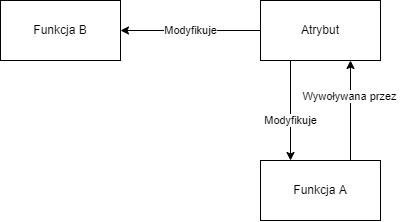
\includegraphics{attribute_function_dependency.png}
\end{figure}

\subsubsection{Funkcje specjalne}
\label{design:attributes:special_functions}

Funkcje specjalne atrybutów, służą do reagowania na użycie obiektu, z którym powiązana jest adnotacja.
Ma to ułatwić tworzenie analizatorów.
Tworząc na przykład odpowiednik niezmiennika \lstinline{const} z C++, programista musi znaleźć wszystkie użycia zmiennej.
W obecnej wersji C-=- istnieją następujące funkcję specjalne:
\begin{itemize}
	\item Funkcje\begin{itemize}
		\item \lstinline{onCall}
	\end{itemize}
	\item Zmienne\begin{itemize}
		\item \lstinline{onDeclare}
		\item \lstinline{onReference}
	\end{itemize}
\end{itemize}
%todo: more, this is an important part of the thesis
Ponadto, każdy cel ma ze sobą powiązaną funkcję \lstinline{attach}.
Ta procedura jest wywoływana, kiedy nagłówek obiektu został stworzony.
Na przykład dla funkcji, dzieje się to kiedy kompilator zebrał jej nazwę, parametry oraz typ zwracany.
Dzieje się to na etapie \lstinline{confirm} przetwarzania pliku źródłowego, który został dokładniej opisany w rozdziale \ref{implementation:source_processing_phases}.

Celem funkcji \lstinline{attach} jest modyfikowanie metadanych obiektu, zanim będą one potrzebne.
Ta procedura to jedyny czas, kiedy kod użytkownika może zmieniać dane używane przy wybieraniu przeciążenia funkcji.
To ograniczenie gra dużą rolę przy zapewnieniu deterministycznego wyniku kompilacji.
Proces wyboru przeciążenia funkcji w C-=-1, jest złożony i został dokładniej opisany w rozdziale \ref{Function_overload_resolution}.


\subsection{Reprezentacja pośrednia}\label{reprezentacja_posrednia}
Programista C-=-1 może analizować oraz modyfikować reprezentację pośrednią swojego programu w czasie kompilacji.
C-=-1 Intermidiate Representation, w skrócie CIR jest nieznacznie uproszczoną wersją języka, reprezentowaną jako struktura danych.
Użytkownik wchodzi w interakcje z CIR za pomocą zestawu interfejsów opisanych w załączniku 1.
Wszystkie typy instrukcji oraz wyrażeń mają ze sobą powiązany konkretny typ.
Wyjątkiem jest \lstinline{ScopeTerminationStatement}, który nie jest powiązany z żadną instrukcją pisaną przez użytkownika.
Instrukcja zakończenia zakresu jest wstawiana przez kompilator na koniec każdej instrukcji złożonej i jest odpowiedzialna za wywołanie destruktorów zmiennych lokalnych (opisane w rozdziale \ref{classes_definition}).

\begin{minipage}{\linewidth}
	\begin{lstlisting}[
		numbers=left,
		firstnumber=0,
		caption={Kod w C++ zawierający przeciążoną funkcję},
		aboveskip=0pt,
		label={lst:cpp_overloaded_function}
	]
int add(int a, int b);
float add(float a, float b);
int main() {
  add(1, 2);
  add(1.0, 2.0);
}
	\end{lstlisting}
\end{minipage}

CIR jest najbardziej zbliżona do drzewa AST programu.
Jednak, zamiast bazować na składni programu, ta struktura danych opiera się na jego semantyce.
Rozważmy fragment kodu C++ w listingu \ref{lst:cpp_overloaded_function}.
Zawiera on dwa przeciążenia funkcji \lstinline{add}: jedno przyjmujące dwa parametry \lstinline{int} a drugie przyjmujące \lstinline{float}.
Z punktu widzenia drzewa AST, wywołania w liniach 3 i 4, różnią się wyłącznie przekazywanymi stałymi.
Identyfikator funkcji (w tym wypadku \lstinline{add}) nie wskazuje jej w sposób unikatowy \cite{ISO:cpp20}, kompilator musi dokonać wyboru przeciążenia na podstawie przekazywanych parametrów \cite{cpp:function_overload_frontend}.

CIR, zamiast opierać się na tekście źródłowym, składa się z odniesień do konkretnych elementów programu.
Tak więc w kontekście przykładu z listingu \ref{lst:cpp_overloaded_function}, obiekty w modelu odpowiadające liniom 3 i 4 zawierałyby jednakowe wskazania na funkcje.
CIR, w przeciwieństwie do drzewa AST składa się więc wyłącznie z informacji o znaczeniu semantycznym, nie składniowym.

Robiąc przegląd literatury, nie znaleziono struktury danych o charakterystyce zbliżonej do CIR.
Zaproponowano więc nowy termin: reprezentacja semantyczna.
Opisuje on strukturę danych, opisującą program, składającą się wyłącznie z informacji o znaczeniu semantycznym.
Reprezentacja semantyczna zawiera komplet informacji potrzebnych do zrozumienia programu.
Operacje takie jak wybieranie przeciążenia, po jego skonstruowaniu, są zbędne.

\subsection{Zarządzanie pamięcią}
\label{memory_management}
Zarządzanie pamięcią w C-=-1 jest oparte na C++11. W 2011 do biblioteki standardowej zostały wprowadzone nowe typy 'inteligentnych wskaźników': \lstinline{unique_ptr}, \lstinline{shared_ptr} oraz \lstinline{weak_ptr}\cite{ISO:2012:III}.
Miały one na celu wprowadzenie do języka mechanizmów umożliwiających tanie i automatyczne zarządzanie pamięcią oraz semantyczne podkreślenie relacji między obiektami.
Korzystając z doświadczeń C++, gdzie te wskazania stały się zalecanym sposobem zarządzania pamięcią\cite{cpp:core_guidelines}, inteligentne wskazania są integralną częścią C-=-1.
\subsection{Struktura pakietu}\label{struktura_paczki}
Projekt w języku C-=-1 jest identyfikowany przez plik manifestu (ang: manifest) o rozszerzeniu \lstinline{.mn}. 
Zawiera on metadane na temat pakietu: unikatowy identyfikator, dane autora, zależności i tym podobne.
Pliki źródłowe mają rozszerzenia \lstinline{.cm}. W tym samym folderze co manifest znajduje się folder \lstinline{src}. Kompilator zakłada, że wszystkie pliki o rozszerzeniu \lstinline{.cm} będące jego potomkami należą do projektu definiowanego przez manifest.
W pliku \lstinline{.mn} zdefiniowane są metadane na temat pakietu takie jak autor, wersja czy zależności. Ten aspekt języka jest modelowany na bazie Rust i pliku \lstinline{cargo.toml}.
